\cotefile{10}
\scanpage{123}
\mspage{122}

% source lines 1--20
$\handwritten{\pi}_i^{\handwritten{2}}=\handwritten{\pi}_i,\handwritten{\pi}_i\handwritten{\pi}_j=0$ for $i\handwritten{\ne}j$, $\handwritten{\sum_i\pi}_i=1$. The datum of a $\unsure{\otimes|\Omega}$-structure on $C$ \rlap{c}implying the data a)b),and these compatible with the functor $C\handwritten{\to}D$ (for $c=\mathrm{id}$),is then equivalent to a unital associative algebra structure on $A$, \rlap{p}compatible with the coalgebra structure, and for which $A\handwritten{\to}k\handwritten{[}T,T^{-1}\handwritten{]}$ is a homomorphism of \unsure{\rlap{\begin{tikzpicture}[x=1em,y=1em,baseline=0pt]\draw (.28,.72) .. controls (.26,.58) and (.30,.48) .. (.34,.32);\draw (.56,.34) .. controls (.66,.48) and (.81,.43) .. (.75,.30) .. controls (.71,.21) and (.66,.17) .. (.65,.11);\end{tikzpicture}}a|a|À}lgebras. How is the fact expressed that \deleted{$C\unsure{\to}D$ is} on $C$ there is a symmetry structure \deleted{such} preserved by the functor $C\handwritten{\to}D$ (and $\unsure{\mathbb{c}|c}$ chosen above) ? One can first express the preceding \inserted{\handwritten{$\otimes$}\handwritten{\begin{tikzpicture}[x=.4cm,y=.4cm,baseline=-.2ex]\draw (0,-.35) .. controls (.10,-.05) and (.20,.20) .. (.38,.42);\end{tikzpicture}}}-structure by a diagonal map of $U$ satisfying $\handwritten{\Delta}(\handwritten{\pi}_i)=\handwritten{\sum}_{j+k=i}\handwritten{\pi}_j\otimes\handwritten{\pi}_k$. \rlap{C}The condition sought \deleted{amounts to saying that if $M$ is a $U$-module of degree $i$, \unsure{\rlap{N}i|N}.e. such that ${}_iM=M$, and $N$ of degree $j$ i.e. ${}_jN=N$, then the\rlap{'} isomorphism $x\otimes y\quad(-1)^{ij}y\otimes x$ from $M\otimes_kN$ onto $N\otimes_kM$ is compatible with the operations of $U$} is this: if we grade $U$ by ``degree of operators in graded objects'' i.e. \deleted{$U^i\unsure{=\pi_j|=\sum_j}$} these quotients $U_{\handwritten{\alpha}}$ by $U_{\handwritten{\alpha}}^i=\handwritten{\widehat{\sum}\pi}_{i+j}U_{\handwritten{\alpha}}\handwritten{\pi}_i$, then the diagonal map becomes \uline{anti}commutative i.e. the mu\rlap{l}t\rlap{l}tiplication of $A$ \deleted{respects} is \uline{anticommutative}. (It would be appropriate to prove that the grading of $A$\inserted{i.e. of $U$\handwritten{\begin{tikzpicture}[x=.45cm,y=.45cm,baseline=-.2ex]\draw (0,-.35) .. controls (-.06,.05) and (.18,.13) .. (.40,.15)--(2.0,.15) .. controls (2.22,.16) and (2.40,.20) .. (2.41,.42);\end{tikzpicture}}} allows one to recover th\rlap{e}e \deleted{functor \unsure{to the|of the}} \rlap{f}grading on the forgetful functor,\margin{to be checked, \handwritten{(arbitrary \unsure{group} \unsure{of|of the} classes for \unsure{grading|grading} ?)}} i.e. the $\handwritten{\pi}_i\handwritten{\in}U$ i.e. $A\handwritten{\to}k\handwritten{[}T,T^{-1}\handwritten{]}$, and that the grading of $A$ \deleted{is not} can be chosen arbit\rlap{r}ra\rlap{r}rily, with the sole condition, in any case necessary\deleted{s}, that $A$ be anticommutative and the diagonal homomorphism \rlap{is}\handwritten{\unsure{be}} compatible with the gradings).

% source lines 21--27
\handwritten{9\unsure{/|)}} Whatever the structures a)\deleted{b)}c) in play\inserted{(b) -the unit - being \rlap{fixed}\handwritten{\unsure{fixed}}\handwritten{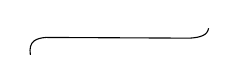
\begin{tikzpicture}[x=.45cm,y=.45cm,baseline=-.2ex]\draw (0,-.35) .. controls (-.06,.04) and (.17,.12) .. (.44,.14)--(4.5,.12) .. controls (4.8,.14) and (5.0,.20) .. (5.03,.40);\end{tikzpicture}}}, the group of $\otimes$-automorphisms of the \deleted{fibre} ``forgetful'' functor is independent of them, it is the group of $\unsure{\mathbb{g}|g}\handwritten{\in}U$ such that $\handwritten{\Delta}(g)=g\otimes g$ and of augmentation 1,\inserted{\handwritten{(i.e. the unital homomorphisms $\unsure{g|q}:A\to k$)}\handwritten{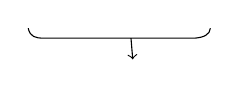
\begin{tikzpicture}[x=.45cm,y=.45cm,baseline=-.2ex]\draw (0,.28) .. controls (.05,.04) and (.20,.0) .. (.44,.0)--(4.7,.0) .. controls (4.95,.02) and (5.13,.10) .. (5.14,.28);\draw[->] (2.9,0)--(2.95,-.60);\end{tikzpicture}}}\unsure{(}NB this last condition for\unsure{$\mathbb{m}$|m}ulates condition b) of 3º). Replacing $k$ by an arbitrary algebra, one again finds an \deleted{funct} affine monoid scheme over $k$, but which in general will not make it possible to reconstitu\deleted{t}te the situation entirely. \deleted{(give example} One must analyse more closely
